%~~~~~~~~~~~~~~~~~~~~~~~~~~~~~~~~~~~~~~~~~~~~~~~~~~~~~~~~~~~~~~~~~~~~~
%    File      : ppi_metodologia
%~~~~~~~~~~~~~~~~~~~~~~~~~~~~~~~~~~~~~~~~~~~~~~~~~~~~~~~~~~~~~~~~~~~~~

Detalhar a metodologia que será utilizada para o desenvolvimento do plano de pesquisa individual. Como referência, apresenta-se o \MAIA\ -- \maia, utilizado pelo \inova.

A metodologia utilizada para o desenvolvimento do projeto utilizará o \MAIA\ (\maia) \cite{costa_um_2010}, cujo conceito simplificado é apresentado na \autoref{fig:maia}.

\begin{figure}[H]
  \centering
  \caption[\maia]{\MAIA\ -- \maia}\label{fig:maia}
  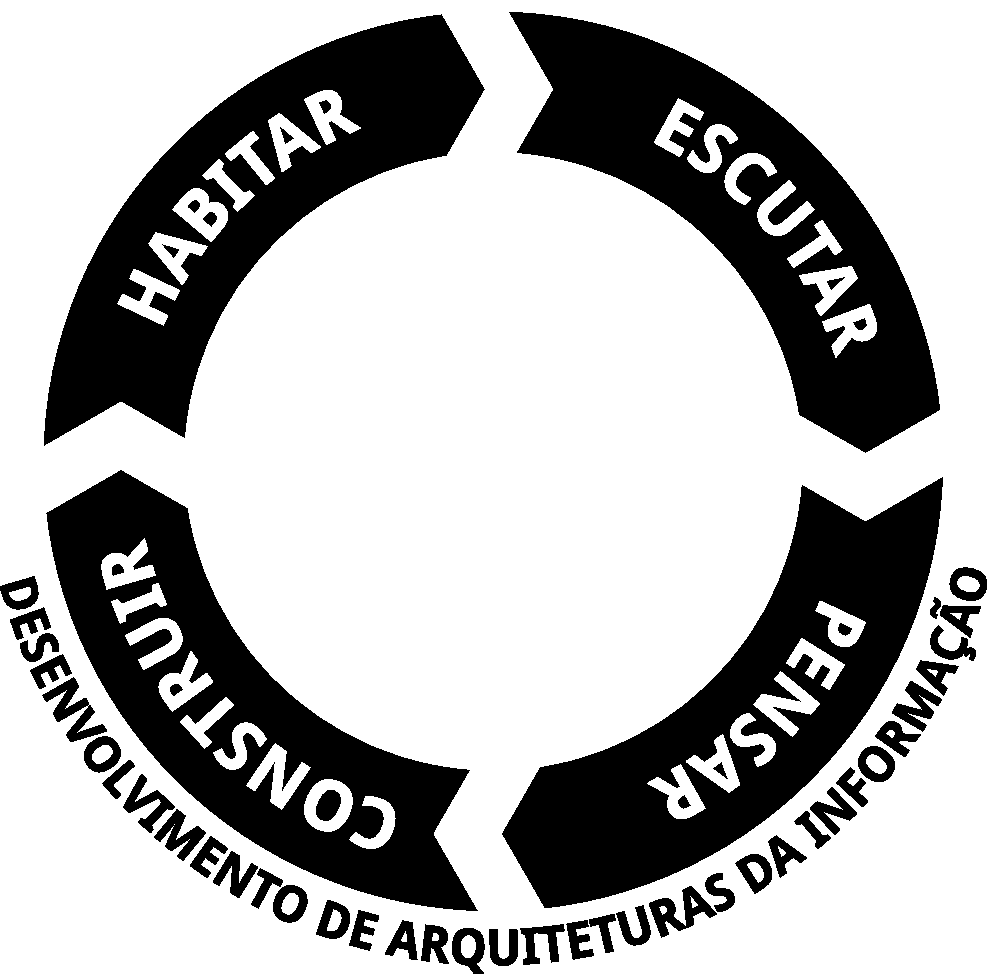
\includegraphics[width=0.4\linewidth,frame=0.5pt 5pt]{img/maia}
  \fonte{Equipe de pesquisa -- \textsc{cpai} (2016)}
\end{figure}

O Escutar, o Pensar, o Construir e o Habitar são momentos de atuação do sujeito sobre um espaço de informação. O Escutar e o Pensar são momentos voltados para os aspectos abstratos deste espaço. O Construir e o Habitar são momentos voltados para os aspectos concretos. O Escutar é o momento que concentra as percepções do espaço de informação. O Pensar concentra a modelagem hermenêutica de um espaço de informação. O Construir reúne as ações de manipulação dos elementos de um espaço de informação. O Habitar é o momento no qual o sujeito usa o espaço de informação percebido, modelado e aperfeiçoado com suas intenções. A configuração dos elementos em um espaço de informação é denominado de \AI\ (\ai).


\section{Percurso Metodológico}\label{sec:percurso_metodologico}

Etapas necessárias para o desenvolvimento do plano. Segue referência:

Esta pesquisa possuirá abordagem explicativa e qualitativa. Os procedimentos técnicos adotados serão bibliográfico, estatístico e estudo de caso. O percurso metodológico seguirá o seguinte caminho:

\begin{alineas}
    \item Levantamento bibliográfico e análise nas áreas relevantes;
    
    \item Investigação qualitativa para a análise da formação do juízo de valor em usuários de repositórios digitais e as circunstâncias de uso desses repositórios;
    
    \item Estabelecimento de relações entre as abordagens teóricas e a investigação qualitativa, buscando encontrar pontos de convergência e distanciamento entre a visão conceitual e a aplicação pragmática;

    \item Validação do modelo proposto em base empírica.
\end{alineas}

